
% !TEX program = lualatex
% Compile (recommended):
%   lualatex digital_euro_thesis.tex
%   biber digital_euro_thesis
%   lualatex digital_euro_thesis.tex
%   lualatex digital_euro_thesis.tex
%
% Notes:
% - This is a full thesis-style draft in one file (self-contained, incl. BibTeX via filecontents).
% - Replace placeholders like <Your Name>, <University>, etc.
% - Page count depends strongly on formatting, figures, and institutional template requirements.

\documentclass[12pt,a4paper]{report}

% -------------------- Packages --------------------
\usepackage[a4paper,margin=1in]{geometry}
\usepackage{setspace}
\onehalfspacing

\usepackage[T1]{fontenc}
\usepackage{lmodern}
\usepackage{microtype}
\usepackage{graphicx}
\usepackage{booktabs}
\usepackage{tabularx}
\usepackage{longtable}
\usepackage{multirow}
\usepackage{array}
\usepackage{amsmath,amssymb}
\usepackage{siunitx}
\usepackage{enumitem}
\usepackage{hyperref}
\usepackage{csquotes}
\usepackage{float}
\usepackage{caption}
\usepackage{subcaption}
\usepackage{listings}
\usepackage{xcolor}
\usepackage{algorithm}
\usepackage{algpseudocode}
\usepackage{tikz}
\usetikzlibrary{arrows.meta,positioning,shapes.geometric,fit,calc}
\usepackage{pgfplots}
\pgfplotsset{compat=1.18}

% -------------------- Bibliography (APA) --------------------
\usepackage[backend=biber,style=apa,sortcites=true,natbib=true]{biblatex}
\DeclareLanguageMapping{english}{english-apa}

\begin{filecontents*}{references.bib}
@report{ecb_costs_2025,
  author       = {{European Central Bank}},
  title        = {A view on recent assessments of digital euro investment costs for the euro area banking sector},
  year         = {2025},
  month        = oct,
  institution  = {European Central Bank},
  type         = {Report},
  note         = {ECB analysis of banking-sector implementation cost estimates and synergy/cost-mutualisation scenarios.}
}

@report{pwc_coststudy_2025,
  author       = {{PricewaterhouseCoopers}},
  title        = {Digital Euro Cost Study},
  year         = {2025},
  month        = jun,
  institution  = {PricewaterhouseCoopers},
  type         = {Industry study},
  note         = {Commissioned by European Credit Sector Associations; panel of 19 retail banks.}
}

@report{ecb_closing_report_2025,
  author       = {{European Central Bank}},
  title        = {Preparation phase of a digital euro: Closing report},
  year         = {2025},
  institution  = {European Central Bank},
  type         = {Report},
  note         = {End-of-phase report including rulebook and innovation platform results.}
}

@report{ecb_rdg_progress_2025,
  author       = {{European Central Bank}},
  title        = {Update on the work of the digital euro scheme's Rulebook Development Group},
  year         = {2025},
  month        = oct,
  institution  = {European Central Bank},
  type         = {Progress report},
  note         = {Status update on the digital euro scheme rulebook development (RDG).}
}

@report{ecb_innovation_annex_2025,
  author       = {{European Central Bank}},
  title        = {DESP Experimentation Portal -- User Guide (Innovation Platform Annex)},
  year         = {2025},
  month        = sep,
  institution  = {European Central Bank},
  type         = {Technical annex},
  note         = {Experimentation portal (REST/gRPC) guidance and innovation platform annex.}
}

@report{eba_guide_2023,
  author       = {{Euro Banking Association (EBA)}},
  title        = {The Digital Euro -- A Guide for Banks: Possible ways forward and the role of banks in the digital euro},
  year         = {2023},
  institution  = {Euro Banking Association},
  type         = {Industry guide},
  note         = {Digital Currencies \& Smart Payments Working Group.}
}

@report{cipa_rilevazione_it_2025,
  author       = {{CIPA}},
  title        = {Rilevazione sull'IT nel settore bancario italiano: Profili economici e organizzativi},
  year         = {2025},
  institution  = {CIPA (in cooperation with Banca d'Italia)},
  type         = {Survey report},
  note         = {IT cost and organisational survey for the Italian banking sector (RILECO-2024).}
}

@online{ecb_digital_euro_page,
  author  = {{European Central Bank}},
  title   = {Digital euro},
  year    = {2025},
  url     = {https://www.ecb.europa.eu/euro/digital_euro/html/index.en.html},
  urldate = {2026-01-24}
}

@online{eu_council_2025_digital_euro_position,
  author  = {{Council of the European Union}},
  title   = {Single currency: Council agrees position on the digital euro and on strengthening the role of cash},
  year    = {2025},
  month   = dec,
  day     = {19},
  url     = {https://www.consilium.europa.eu/en/press/press-releases/2025/12/19/single-currency-council-agrees-position-on-the-digital-euro-and-on-strengthening-the-role-of-cash/},
  urldate = {2026-01-24}
}

@online{bundesbank_digital_euro_2025,
  author  = {{Deutsche Bundesbank}},
  title   = {Digitaler Euro auf einen Blick},
  year    = {2025},
  url     = {https://www.bundesbank.de/de/aufgaben/unbarer-zahlungsverkehr/digitaler-euro/digitaler-euro-auf-einen-blick/auf-einen-blick-903500},
  urldate = {2026-01-24}
}

@online{db_digital_euro_2025,
  author  = {{Deutsche Bank}},
  title   = {The Digital Euro: A New Era for the European Monetary System},
  year    = {2025},
  month   = dec,
  day     = {11},
  url     = {https://www.db.com/news/detail/20251211-the-digital-euro-a-new-era-for-the-european-monetary-system?language_id=1},
  urldate = {2026-01-24}
}

@online{kpmg_impl_starts_here_2025,
  author  = {{KPMG}},
  title   = {The Digital Euro: Implementation starts here},
  year    = {2025},
  url     = {https://kpmg.com/xx/en/our-insights/ecb-office/kpmg-european-central-bank-office-fs/the-digital-euro-implementation-starts-here.html},
  urldate = {2026-01-24}
}
\end{filecontents*}

\addbibresource{references.bib}

% -------------------- Listings --------------------
\lstdefinestyle{json}{
  basicstyle=\ttfamily\small,
  breaklines=true,
  frame=single,
  columns=fullflexible,
  keepspaces=true
}

% -------------------- Document --------------------
\title{\textbf{Implementation Models for Banks in the Context of the Digital Euro}\\
\vspace{0.5em}\large A technical and organisational thesis on integration architectures, shared services, and bank-tier-specific implementation strategies}
\author{<Your Name> \\ <Department / Faculty> \\ <University>}
\date{\today}

\begin{document}
\pagenumbering{roman}
\maketitle

\chapter*{Abstract}
The potential introduction of a retail digital euro introduces a new payment rail whose operational model combines Eurosystem-provided scheme components with bank- or payment service provider (PSP)-implemented distribution, customer servicing, and compliance capabilities. This thesis develops a technical reference architecture and a set of bank-tier-specific implementation models (in-house, hybrid, outsourced) for integrating the digital euro into existing bank payment ecosystems. The work is grounded in official Eurosystem documentation (rulebook development and preparation-phase materials), the Eurosystem innovation platform/experimentation portal interfaces, and industry cost studies. It proposes a modular decomposition of affected bank components (channels, payment hubs, customer identity, liquidity, compliance, acceptance infrastructure), distinguishes components that can be mutualised across PSPs (shared integration) from those that should remain bank-specific, and evaluates architectural patterns (monolithic, modular monolith, microservices/event-driven) in terms of time-to-market, cost, resilience, and regulatory fit. A multi-criteria decision analysis (MCDA) and scenario-based cost model are used to map appropriate implementation strategies to bank tiers defined by size and operational complexity. The thesis concludes with actionable blueprints and a migration roadmap for banks and PSP consortia, emphasising cost mutualisation opportunities and robust governance aligned with the digital euro scheme rulebook.

\chapter*{Keywords}
Digital euro; CBDC; payment systems; banking architecture; interoperability; shared services; outsourcing; microservices; access gateway; rulebook; cost mutualisation.

\tableofcontents
\listoffigures
\listoftables

\chapter*{Abbreviations}
\begin{longtable}{@{}p{0.18\textwidth}p{0.75\textwidth}@{}}
\toprule
\textbf{Term} & \textbf{Meaning} \\ \midrule
CBDC & Central Bank Digital Currency \\
ECB & European Central Bank \\
Eurosystem & ECB + national central banks of the euro area \\
PSP & Payment Service Provider \\
DESP & Digital Euro Service Platform (term used for Eurosystem service platform) \\
DCA & Dedicated Cash Account (liquidity account concept for intermediaries) \\
API & Application Programming Interface \\
HSM & Hardware Security Module \\
DORA & Digital Operational Resilience Act \\
AML/CFT & Anti-Money Laundering / Countering the Financing of Terrorism \\
KYC & Know Your Customer \\
SCA & Strong Customer Authentication \\
POS & Point of Sale \\
ATM & Automated Teller Machine \\
\bottomrule
\end{longtable}

\cleardoublepage
\pagenumbering{arabic}

% ============================================================
\chapter{Introduction}
\section{Context and motivation}
The digital euro is envisaged as a digital form of central bank money, complementing cash and enabling electronic payments in shops, online, and peer-to-peer across the euro area \parencite{ecb_digital_euro_page}. Its introduction is framed as a strategic response to shifts in the payment landscape (including the growing role of non-European payment infrastructures) and aims to preserve the role of central bank money as an anchor for the payment system \parencite{ecb_digital_euro_page}. In parallel, EU co-legislators have advanced legal-framework discussions; for example, the Council of the EU agreed a negotiating position that emphasises that a digital euro would complement cash and be usable across the euro area \parencite{eu_council_2025_digital_euro_position}.

From a bank/PSP perspective, the digital euro is not a mere ``new instrument'' added to existing channels. Rather, it introduces a new interoperability surface (to the Eurosystem service platform) and a new set of scheme rules, technical standards, operational procedures, and customer-service obligations. Implementation decisions will materially affect cost, delivery risk, and the ability to reuse resulting capabilities for private-sector payment innovation (e.g., pan-European wallet propositions). A central challenge is that banks are heterogeneous: they differ in IT maturity, channel footprints, sourcing strategies, and governance structures. Consequently, a one-size-fits-all integration approach is unlikely to be cost-optimal or operationally resilient.

\section{Problem statement}
Banks must integrate the digital euro into existing payment ecosystems while maintaining service continuity, security, compliance, and cost discipline. The integration touches multiple layers: customer channels (mobile apps, cards, branch/ATM), payment processing and orchestration, customer identity and access management, liquidity/funding mechanics, compliance and risk controls, reporting, and merchant acceptance infrastructure. Industry studies suggest substantial investment may be required if implemented in a stand-alone or non-mutualised manner \parencite{pwc_coststudy_2025}. At the same time, Eurosystem assessments highlight significant potential for cost mutualisation through shared solutions and external synergies, implying that banks need not implement digital euro capabilities entirely on their own \parencite{ecb_costs_2025}.

\section{Research objectives and questions}
Guided by the attached research outline (user-provided), this thesis addresses the following research questions (RQs):

\begin{enumerate}[label=\textbf{RQ\arabic*:},leftmargin=2.5em]
\item How can banks technically integrate the digital euro into existing architectures, and what are the principal integration patterns?
\item Which capabilities are provided by the Eurosystem (scheme/DESP) versus those to be implemented by intermediaries (banks/PSPs)?
\item Which bank/PSP modules are affected by digital euro integration, and how can these be decomposed into reusable components?
\item Which integration components can be mutualised/shared across PSPs (software and hardware), and which must remain bank-specific?
\item Which implementation model (in-house, hybrid, outsourced) is appropriate for different bank tiers, considering cost, risk, and time-to-market?
\end{enumerate}

\section{Contributions}
The thesis makes five contributions:
\begin{enumerate}[leftmargin=2.2em]
\item A \textbf{rulebook-aligned reference architecture} that maps scheme functions to bank modules and integration interfaces.
\item A \textbf{bank/PSP module impact model}, linking functional domains (access, transaction, liquidity, offline, acceptance) to internal components.
\item A \textbf{shared vs. dedicated integration taxonomy} across software and hardware (e.g., gateways, offline devices, acceptance utilities).
\item A \textbf{bank-tier-specific implementation model matrix} (in-house / hybrid / outsourced) with MCDA scoring and decision rules.
\item A \textbf{scenario-based cost and resource analysis} synthesising public cost studies and synergy mechanisms.
\end{enumerate}

\section{Scope and assumptions}
The work focuses on retail digital euro distribution by banks and PSPs in the euro area context. It is concerned with integration architecture and operating models rather than macroeconomic impacts. Where rulebook details remain under development, the thesis uses published preparation-phase and rulebook development updates and clearly states assumptions \parencite{ecb_closing_report_2025,ecb_rdg_progress_2025}.

% ============================================================
\chapter{Background: Digital euro scheme and platform}
\section{Scheme governance and rulebook structure}
The Eurosystem has organised rulebook development through a Rulebook Development Group (RDG), aiming to provide a single set of rules and standards for intermediaries and the ecosystem \parencite{ecb_costs_2025,ecb_rdg_progress_2025}. The preparation phase documentation indicates that the scheme rulebook is intended to specify roles, responsibilities, operational procedures, and technical standards necessary for uniform implementation \parencite{ecb_closing_report_2025}.

\subsection{Functional domains}
In order to align the thesis with the scheme's structure, we use the following domain breakdown as organising principle throughout Chapters 4--9:
\begin{itemize}
\item \textbf{Access management}: onboarding, authentication, device binding, credential lifecycle, and access policies.
\item \textbf{Transaction management}: payment initiation, authorisation, execution, reversals, dispute primitives, and status tracking.
\item \textbf{Liquidity management}: DCA funding/defunding, limits enforcement, and treasury interfaces.
\item \textbf{Alias and reference data}: lookup/portability, identifiers, and scheme reference data.
\item \textbf{Settlement and reporting}: settlement-related interactions, fee/reporting interfaces (including Eurosystem-provided functions).
\item \textbf{Offline and conditional/value-added features}: offline synchronisation, conditional payments, and programmable services layered on acceptance standards.
\end{itemize}

\section{Intermediary role and the ``access gateway'' concept}
Industry guidance highlights that intermediaries (banks/PSPs) connect to the digital euro service platform through an \emph{access gateway} that acts as a single point of contact, abstracting/hiding backend components behind a unified interface \parencite{eba_guide_2023}. This design aligns with the principle of reducing integration coupling by providing a stable interface boundary between intermediaries and the Eurosystem platform, supporting both interoperability and evolvability.

\section{Digital euro channels and acceptance ecosystem}
The digital euro is intended to support payments in physical POS, e-commerce, and P2P contexts \parencite{ecb_digital_euro_page}. National central banks communicate the project as a complement to cash with broad usability and strong safety properties \parencite{bundesbank_digital_euro_2025}. From an intermediary perspective, channel integration involves:
(i) consumer-facing wallets or wallet capabilities integrated into existing banking apps,
(ii) merchant acceptance enablement (POS terminal updates, payment pages, QR/NFC interaction),
and (iii) cash-like access paths such as branch/ATM interfaces for onboarding and funding/defunding \parencite{pwc_coststudy_2025}.

\section{Innovation platform and experimentation portal}
The preparation phase included an innovation platform in which market participants tested use cases and interfaces, including conditional-payment features and e-commerce/payment initiation scenarios \parencite{ecb_closing_report_2025,ecb_innovation_annex_2025}. The experimentation portal supports both synchronous REST APIs and gRPC interfaces; implementation specifications include REST due to market preference while supporting gRPC for broader ecosystem compatibility \parencite{ecb_innovation_annex_2025}.

% ============================================================
\chapter{Related work and literature review}
\section{CBDC integration architectures}
CBDC technical literature commonly distinguishes between (a) core ledger and issuance infrastructure, typically central bank-operated, and (b) intermediary distribution layers providing wallets, KYC, customer service, and value-added features. For the digital euro, this aligns with the access-gateway model and intermediary responsibilities as described in industry guidance and Eurosystem documents \parencite{eba_guide_2023,ecb_closing_report_2025}.

\section{Payment industry mutualisation}
The payment industry historically relies on shared infrastructures (clearing/settlement utilities, scheme processors, shared compliance tooling). The ECB cost assessment explicitly notes that banks already use shared solutions for payment channels, accounts, compliance, and operational support, and argues similar approaches can be applied to digital euro integration \parencite{ecb_costs_2025}. This provides a foundation for modelling shared vs. dedicated modules in this thesis.

\section{Cost evidence and concerns}
A prominent industry study estimates that participating banks could face over \EUR{2} billion in introduction costs (panel of 19 banks), with an extrapolated euro-area figure of \EUR{18} billion, and indicates that the technical layer constitutes around 75\% of cost \parencite{pwc_coststudy_2025}. In contrast, the ECB cost note suggests that once cost mutualisation and synergies are accounted for, total costs could fall in a range of \EUR{4}--\EUR{5.77} billion over four years \parencite{ecb_costs_2025}. This gap motivates systematic identification of mutualisable components and bank-tier-specific operating models.

\section{Gap analysis}
Existing publications provide (i) high-level descriptions of digital euro objectives and status \parencite{ecb_digital_euro_page,eu_council_2025_digital_euro_position}, (ii) industry guidance on intermediary roles and access gateway concepts \parencite{eba_guide_2023}, and (iii) cost estimates with different assumptions \parencite{pwc_coststudy_2025,ecb_costs_2025}. However, there is limited publicly available work translating these into an actionable, rulebook-aligned reference architecture and decision framework mapping implementation models to bank tiers. This thesis addresses that gap.

% ============================================================
\chapter{Methodology}
\section{Research design}
The thesis combines \textbf{design science} and \textbf{applied systems engineering}. The artefacts are (a) a reference architecture, (b) implementation model matrix, and (c) decision and cost analysis tools. Evidence is derived from document analysis of Eurosystem publications and industry studies, and synthesis into architectural patterns.

\section{Data sources}
Primary sources include:
\begin{itemize}
\item Eurosystem/ECB rulebook and preparation-phase materials \parencite{ecb_closing_report_2025,ecb_rdg_progress_2025,ecb_innovation_annex_2025};
\item Industry guidance for banks on the digital euro \parencite{eba_guide_2023};
\item Public cost studies and cost-synergy analysis \parencite{pwc_coststudy_2025,ecb_costs_2025};
\item Sector IT survey evidence for outsourcing and IT spend profiles (contextual) \parencite{cipa_rilevazione_it_2025}.
\end{itemize}

\section{Analytical framework}
Two complementary analyses are applied:

\subsection{(A) Module decomposition and sharing potential}
We decompose end-to-end digital euro capabilities into modules, then classify each module as:
\begin{itemize}
\item \textbf{Mutualisable}: can be shared across banks/PSPs (e.g., via a utility or vendor) with limited loss of differentiation.
\item \textbf{Group-shared}: mutualisable within a banking group, IPS, or cooperative structure.
\item \textbf{Bank-specific}: must remain within each bank due to customer relationship, risk appetite, data constraints, or strategic differentiation.
\end{itemize}
The ECB cost note provides an analytical basis and empirical synergy factors for market-wide and group-level mutualisation \parencite{ecb_costs_2025}.

\subsection{(B) Multi-criteria decision analysis (MCDA)}
Implementation options (in-house, hybrid, outsourced) are evaluated per bank tier using MCDA with criteria:
time-to-market, CapEx, OpEx, integration risk, security/compliance, operational resilience, vendor lock-in, scalability, and reuse potential.
Weights are selected to reflect typical supervisory and strategic priorities; sensitivity analysis is included.

\section{Bank tiering model}
We define bank tiers in line with size clusters used in cost evidence (assets brackets) \parencite{pwc_coststudy_2025,ecb_costs_2025}:
\begin{itemize}
\item \textbf{Tier 1 (Top)}: total assets $> \EUR{1}$ trillion.
\item \textbf{Tier 2 (Large)}: $\EUR{100}$ billion -- $\EUR{1}$ trillion.
\item \textbf{Tier 3 (Mid)}: $\EUR{30}$ billion -- $\EUR{100}$ billion.
\item \textbf{Tier 4 (Small)}: $< \EUR{30}$ billion.
\end{itemize}
This is a practical proxy for organisational scale, channel footprint (ATM/branch/POS), and engineering capacity.

% ============================================================
\chapter{Technical integration: reference architecture}
\section{High-level integration landscape}
Figure~\ref{fig:ref-arch} provides a rulebook-aligned high-level architecture. Intermediaries integrate via a dedicated \emph{Digital Euro Integration Layer} (DEIL) that encapsulates protocol adapters (REST/gRPC), security controls, and business orchestration, and connects internal systems and channels to the access gateway.

\begin{figure}[H]
\centering
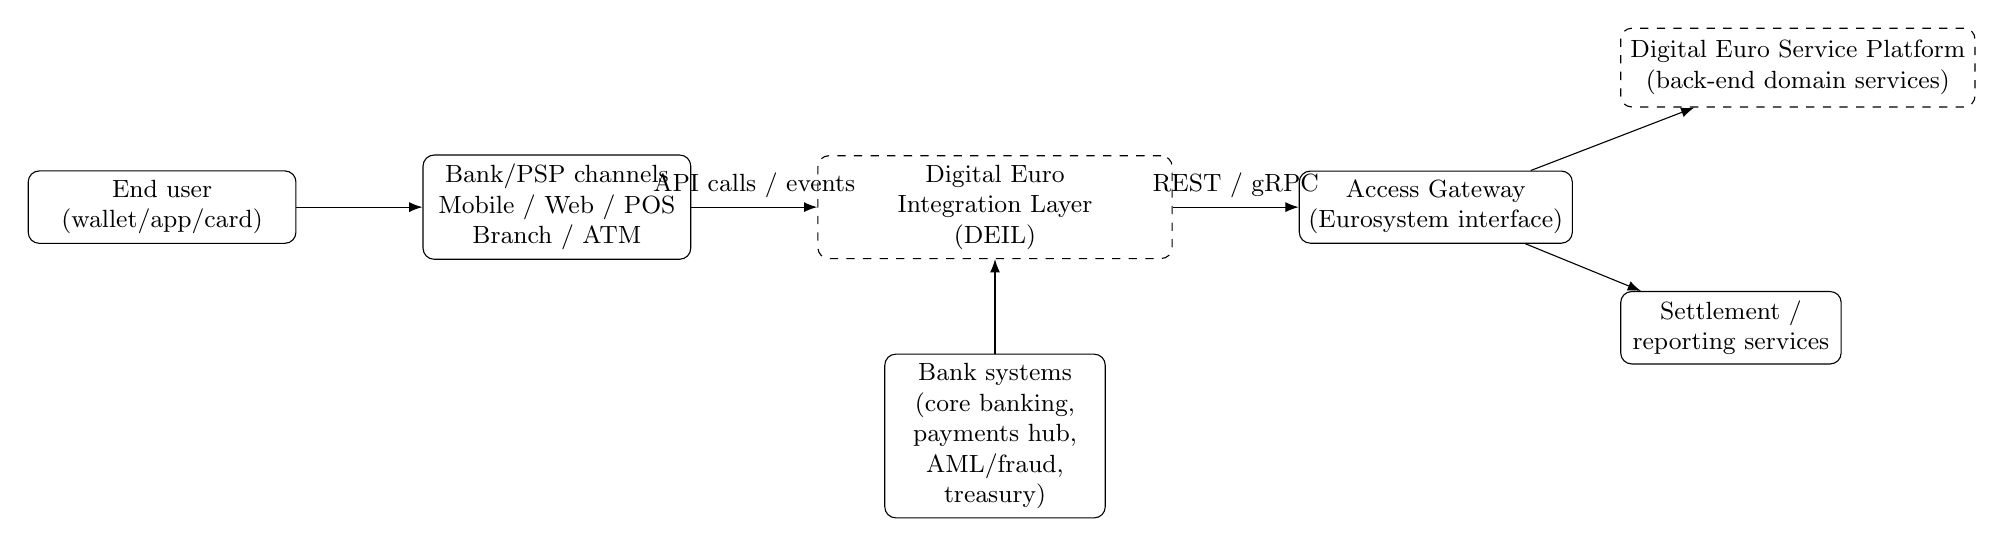
\begin{tikzpicture}[node distance=8mm, font=\small]
\tikzstyle{box}=[draw, rounded corners, align=center, minimum width=34mm, minimum height=8mm]
\tikzstyle{smallbox}=[draw, rounded corners, align=center, minimum width=28mm, minimum height=7mm]
\tikzstyle{cloud}=[draw, rounded corners, align=center, minimum width=45mm, minimum height=10mm, dashed]

\node[box] (cust) {End user\\(wallet/app/card)};
\node[box, right=16mm of cust] (chan) {Bank/PSP channels\\Mobile / Web / POS\\Branch / ATM};
\node[cloud, right=16mm of chan] (deil) {Digital Euro\\Integration Layer\\(DEIL)};
\node[box, right=16mm of deil] (ag) {Access Gateway\\(Eurosystem interface)};

\node[cloud, above right=8mm and 6mm of ag] (desp) {Digital Euro Service Platform\\(back-end domain services)};
\node[smallbox, below right=6mm and 6mm of ag] (sett) {Settlement /\\reporting services};
\node[smallbox, below=12mm of deil] (bankcore) {Bank systems\\(core banking,\\payments hub,\\AML/fraud,\\treasury)};

\draw[-{Latex}] (cust) -- (chan);
\draw[-{Latex}] (chan) -- node[above]{API calls / events} (deil);
\draw[-{Latex}] (deil) -- node[above]{REST / gRPC} (ag);
\draw[-{Latex}] (ag) -- (desp);
\draw[-{Latex}] (ag) -- (sett);
\draw[-{Latex}] (bankcore) -- (deil);
\end{tikzpicture}
\caption{Reference architecture: intermediary integration via a Digital Euro Integration Layer (DEIL) and the access gateway.}
\label{fig:ref-arch}
\end{figure}

\section{Protocol and security interface patterns}
The experimentation portal supports REST and gRPC interfaces; REST is a synchronous interface selected in implementation specifications due to market preference, while gRPC is supported for broader compatibility \parencite{ecb_innovation_annex_2025}. For REST, the portal uses HTTP Basic Authentication and requires request signatures for state-changing methods (e.g., POST/PUT), while GET requests do not require signatures \parencite{ecb_innovation_annex_2025}.

\subsection{Security controls and key management}
A production-grade integration requires layered controls:
\begin{itemize}
\item \textbf{Transport security}: mutual TLS and network segmentation.
\item \textbf{Request authentication}: BasicAuth (or production equivalent) plus signed requests where applicable \parencite{ecb_innovation_annex_2025}.
\item \textbf{Non-repudiation}: signing keys protected by HSMs; auditable signature verification logs.
\item \textbf{Authorisation}: policy enforcement (scopes, roles, device binding) aligned with access management domain.
\item \textbf{Observability}: centralised logging, distributed tracing, anomaly detection.
\end{itemize}

\subsection{Example request-signing envelope (illustrative)}
\begin{lstlisting}[style=json,caption={Illustrative JSON envelope for signed request payloads (conceptual).}]
{
  "header": {
    "requestId": "uuid",
    "timestamp": "2026-01-24T10:15:30Z",
    "clientId": "bank-psp-id",
    "signature": "base64(signature_over_canonical_payload)"
  },
  "body": {
    "operation": "initiatePayment",
    "amount": "10.00",
    "currency": "EUR",
    "payee": { "alias": "merchant-xyz" },
    "payer": { "walletId": "..." }
  }
}
\end{lstlisting}

\section{Functional flows}
\subsection{Online payment flow (conceptual sequence)}
Figure~\ref{fig:seq-online} sketches an online payment flow, abstracting scheme specifics while preserving system responsibilities.

\begin{figure}[H]
\centering
\begin{tikzpicture}[font=\small]
\matrix (m) [matrix of nodes, nodes={anchor=west}, column sep=10mm, row sep=2mm]{
\textbf{User} & \textbf{Bank App} & \textbf{DEIL} & \textbf{Access Gateway} & \textbf{DESP/Back-end} \\
};

% lifelines
\foreach \i/\x in {1/0,2/3.1,3/6.2,4/9.5,5/12.9}{
  \draw[dashed] (\x, -0.6) -- (\x, -6.1);
}

% messages
\draw[-{Latex}] (0, -1.2) -- (3.1, -1.2) node[midway, above]{1. initiate};
\draw[-{Latex}] (3.1, -1.8) -- (6.2, -1.8) node[midway, above]{2. validate \& enrich};
\draw[-{Latex}] (6.2, -2.4) -- (9.5, -2.4) node[midway, above]{3. submit payment};
\draw[-{Latex}] (9.5, -3.0) -- (12.9, -3.0) node[midway, above]{4. authorise/execute};
\draw[-{Latex}] (12.9, -3.6) -- (9.5, -3.6) node[midway, above]{5. status};
\draw[-{Latex}] (9.5, -4.2) -- (6.2, -4.2) node[midway, above]{6. status \& receipt};
\draw[-{Latex}] (6.2, -4.8) -- (3.1, -4.8) node[midway, above]{7. notify};
\draw[-{Latex}] (3.1, -5.4) -- (0, -5.4) node[midway, above]{8. confirm};
\end{tikzpicture}
\caption{Conceptual online payment sequence (high-level).}
\label{fig:seq-online}
\end{figure}

\subsection{Liquidity management and DCA mechanics}
Liquidity management is a first-class domain: intermediaries require funding and defunding mechanisms to manage dedicated liquidity positions, commonly described as a Dedicated Cash Account (DCA). Industry guidance discusses DCA funding/defunding and limit mechanics, including ``waterfall'' and ``reverse waterfall'' flows \parencite{eba_guide_2023}. In implementation, the DEIL should integrate with bank treasury systems and intraday liquidity monitoring.

\subsection{Offline and synchronisation}
Offline functionality adds additional state synchronisation and risk controls. The ECB cost note suggests the offline digital euro is expected to leverage online functionality to a large extent and that add-on cost may be limited, though precise procurement-based costs remain to be validated \parencite{ecb_costs_2025}. From an integration standpoint, offline requires:
\begin{itemize}
\item device secure element management (card/phone secure enclave),
\item risk parameters (offline limits, velocity controls),
\item reconciliation and delayed settlement posting,
\item dispute and double-spend detection mechanisms,
\item incident and fraud handling workflows.
\end{itemize}

\begin{algorithm}[H]
\caption{Offline payment synchronisation (conceptual)}
\begin{algorithmic}[1]
\State \textbf{Input:} local offline transactions $T_{local}$, last sync token $s$
\State Verify device integrity and secure element counters
\State Create reconciliation batch $B \leftarrow \text{canonicalise}(T_{local}, s)$
\State Sign batch: $\sigma \leftarrow \text{Sign}_{HSM/SE}(B)$
\State Submit $(B,\sigma)$ to Access Gateway via DEIL
\State Receive result set $R$ (accepted/rejected, updated counters, new sync token $s'$)
\State Apply outcomes: mark accepted txns settled; quarantine rejected for review
\State Update local state with $s'$ and refreshed limits
\end{algorithmic}
\end{algorithm}

% ============================================================
\chapter{Affected bank/PSP components}
\section{Impact map}
Table~\ref{tab:impact-map} lists key bank modules impacted by digital euro integration, aligned with the PwC ``payment layer model'' decomposition and Eurosystem domain framing \parencite{pwc_coststudy_2025,ecb_rdg_progress_2025}.

\begin{table}[H]
\centering
\caption{Impacted bank/PSP components and primary integration responsibilities}
\label{tab:impact-map}
\begin{tabularx}{\textwidth}{@{}p{0.22\textwidth}X p{0.22\textwidth}@{}}
\toprule
\textbf{Module} & \textbf{Change impact} & \textbf{Primary domain(s)} \\ \midrule
Customer channels (mobile/web) & Digital euro wallet UI/UX, payment initiation, transaction history, notifications, customer support hooks. & Access, Transaction \\
Cards / secure elements & Optional physical form factor, SE provisioning, lifecycle mgmt, offline limits. & Access, Offline \\
POS / e-commerce acceptance & Terminal upgrades, QR/NFC flows, payment pages, merchant onboarding, acquiring alignment. & Transaction, Reference data \\
Branch \& ATM network & Onboarding/offboarding support, funding/defunding services, cash-like accessibility. & Access, Liquidity \\
Payments hub / orchestration & New rail routing, state machine, idempotency, retries, reconciliation, disputes primitives. & Transaction \\
Core banking / accounts & Customer account linking (if applicable), statements, accounting postings, GL, fees. & Transaction, Reporting \\
Treasury / liquidity & DCA funding/defunding, intraday liquidity, limits, monitoring. & Liquidity \\
Risk, fraud, AML/CFT & KYC alignment, transaction monitoring, sanctions screening, fraud controls. & Access, Transaction \\
Data \& reporting & Regulatory reporting, audit trails, operational metrics, incident reporting. & Reporting \\
Integration \& security & Gateway adapter, key mgmt, signing, API version mgmt, certification/testing. & Cross-cutting \\
\bottomrule
\end{tabularx}
\end{table}

\section{Interfaces and integration glue}
The DEIL should be implemented as a bounded context that isolates the rest of the bank from scheme evolution. It typically exposes two northbound interfaces:
\begin{itemize}
\item \textbf{Channel APIs}: SDKs for mobile/web; device provisioning for offline.
\item \textbf{Bank internal integration}: event streams and synchronous calls to payments hub, treasury, AML, CRM.
\end{itemize}
Southbound, it hosts adapters for access gateway REST/gRPC and related security requirements \parencite{ecb_innovation_annex_2025}.

\section{Operational processes impacted}
Beyond technology, banks must adjust processes:
\begin{itemize}
\item customer onboarding/offboarding and customer support,
\item incident management and fraud operations,
\item change management and certification against scheme conformance tests,
\item vendor management and outsourcing controls (DORA-aligned),
\item business continuity and cyber-resilience exercises.
\end{itemize}
The operational layer (fee calculation, reporting/payment statistics, processes) is explicitly represented as part of overall cost and effort in industry studies \parencite{pwc_coststudy_2025}.

% ============================================================
\chapter{Shared vs. dedicated integration components}
\section{Rationale for mutualisation}
The ECB cost analysis emphasises that banks already make extensive use of shared solutions for payment channels, accounts, compliance, and operational support, and argues that digital euro integration can similarly leverage shared infrastructures \parencite{ecb_costs_2025}. It further quantifies that cost mutualisation can materially reduce total investment costs and that banks would not have to implement on a stand-alone basis \parencite{ecb_costs_2025}.

\section{Taxonomy of mutualisable components}
Table~\ref{tab:shared} classifies components by mutualisation potential, including software and hardware/physical infrastructure dimensions.

\begin{table}[H]
\centering
\caption{Shared vs. dedicated components: candidate mutualisation scope}
\label{tab:shared}
\begin{tabularx}{\textwidth}{@{}p{0.27\textwidth}X p{0.22\textwidth}@{}}
\toprule
\textbf{Component} & \textbf{Why it can be shared} & \textbf{Typical host} \\ \midrule
Access gateway adapter (REST/gRPC, signing, versioning) & Standardised protocol and security patterns; economies of scale in certification and upgrades. & Vendor / utility / group IT \\
Conformance testing harness \& sandbox tooling & High fixed cost; reusable across participants; reduces duplicated effort. & Utility / consortium \\
Offline device lifecycle services (SE provisioning, key injection) & Hardware security requires specialised tooling; shared HSM/PKI can reduce cost. & Utility + HSM provider \\
Acceptance utilities (POS/ATM upgrade programs) & Merchants/ATMs often served by shared utilities; aligns with replacement cycles and outsourcing trends. & Acquirer/ATM utility \\
Shared fraud signal exchange (optional) & Cross-bank fraud patterns; shared analytics platform can improve detection. & Consortium \\
Reference data distribution (scheme reference data, alias portability adapters) & Standard data sets and portability workflows benefit from central services. & Utility \\
Bank customer relationship data & Differentiation and privacy constraints; bank-specific. & Bank \\
Bank-specific risk appetite \& AML rules & Local regulation, internal policies and models differ. & Bank \\
Treasury strategy and intraday liquidity & Balance sheet and liquidity policies differ. & Bank \\
\bottomrule
\end{tabularx}
\end{table}

\section{Hardware/physical mutualisation: POS and ATM}
Industry cost evidence shows that acceptance infrastructure and ATM/branch networks are major cost drivers \parencite{pwc_coststudy_2025}. The ECB cost note adjusts ATM upgrade assumptions partly due to the trend toward outsourcing ATMs to independent deployers and utilities and due to existing NFC/QR-enabled ATM footprints, discounting ATM upgrade costs accordingly \parencite{ecb_costs_2025}. This supports the thesis position that hardware upgrades can be mutualised via utilities and coordinated procurement, rather than executed separately by each bank.

% ============================================================
\chapter{Implementation models}
\section{Model definitions}
\subsection{In-house}
The bank builds and operates most of the DEIL and surrounding components, including gateway adapter, orchestration, data and reporting, and often custom channel experiences. It typically uses internal platform engineering capabilities (CI/CD, observability, SRE) and aims for strategic reuse across future payment initiatives.

\subsection{Outsourced}
The bank procures digital-euro-specific capabilities from a specialised provider (or banking group utility), integrating via a thin layer. Outsourcing is consistent with the ECB's focus on external synergies and cost mutualisation (e.g., ``outsourcing to central providers or vendors'') \parencite{ecb_costs_2025}.

\subsection{Hybrid}
The bank keeps differentiating elements (customer channels, risk controls, CRM) while outsourcing commoditised or high-fixed-cost capabilities (gateway adapter, offline provisioning, conformance tooling). Hybrid is often the most practical model, aligning to cost mutualisation and bank-specific differentiation needs.

\section{Architectural patterns}
\subsection{Modular monolith vs. microservices}
\begin{itemize}
\item \textbf{Modular monolith}: faster delivery, simpler operations, strong consistency for payment state machines; risk of scaling bottlenecks if poorly modularised.
\item \textbf{Microservices/event-driven}: better scalability and independent release cycles; higher operational complexity; requires mature DevSecOps and observability.
\end{itemize}
Given the criticality of payment flows, many banks adopt a hybrid: a payments state machine service (high integrity) plus event-driven integration to AML, notifications, reporting.

\subsection{Integration styles}
\begin{itemize}
\item \textbf{API-first synchronous}: suitable for real-time authorisation, channel UX.
\item \textbf{Event-driven}: suitable for monitoring, reconciliation, reporting, fraud signals.
\item \textbf{Batch}: used for end-of-day settlement accounting and regulatory reporting extracts.
\end{itemize}

\section{Bank-tier-specific implementation strategy}
\subsection{Decision matrix}
Table~\ref{tab:tier-strategy} maps recommended implementation models to bank tiers.

\begin{table}[H]
\centering
\caption{Recommended implementation model by bank tier (baseline)}
\label{tab:tier-strategy}
\begin{tabularx}{\textwidth}{@{}p{0.14\textwidth}p{0.18\textwidth}X p{0.18\textwidth}@{}}
\toprule
\textbf{Tier} & \textbf{Typical profile} & \textbf{Recommended model} & \textbf{Rationale} \\ \midrule
Tier 1 & Complex channels, strong engineering, high transaction volumes & In-house or Hybrid & Strategic control, scale benefits, reuse; still outsource commoditised components for efficiency. \\
Tier 2 & Large banks with sizeable channels and constraints & Hybrid & Balance between differentiation and cost mutualisation; focus on reuse and shared gateway/offline services. \\
Tier 3 & Mid-sized banks, limited platform engineering & Hybrid leaning outsourced & Adopt shared gateway adapter and offline provisioning; keep AML/risk integration in-house. \\
Tier 4 & Small banks/LSIs & Outsourced / utility model & Minimise fixed costs; rely on shared providers and central apps where permitted; focus on compliance and customer servicing. \\
\bottomrule
\end{tabularx}
\end{table}

\subsection{MCDA scoring example}
Table~\ref{tab:mcda} provides an illustrative MCDA. Scores are indicative and should be calibrated with institution-specific parameters.

\begin{table}[H]
\centering
\caption{Illustrative MCDA criteria and weights}
\label{tab:mcda}
\begin{tabular}{@{}l S[table-format=1.2] l@{}}
\toprule
Criterion & {Weight} & Notes \\ \midrule
Time-to-market & 0.15 & Faster delivery reduces regulatory/project risk. \\
CapEx (build) & 0.15 & Up-front build costs; impacted by channel footprint. \\
OpEx (run) & 0.10 & Operational burden and SRE staffing. \\
Integration risk & 0.15 & Coupling to core systems and maturity of APIs. \\
Security/compliance fit & 0.15 & AML/KYC, auditability, privacy requirements. \\
Operational resilience & 0.15 & High availability, cyber resilience (DORA-aligned). \\
Vendor lock-in risk & 0.10 & Exit cost and concentration risk. \\
Reuse potential & 0.05 & Leverage for future payment innovations. \\
\bottomrule
\end{tabular}
\end{table}

% ============================================================
\chapter{Cost and resource analysis}
\section{Public cost estimates}
The PwC industry study estimates introduction costs exceeding \EUR{2} billion for 19 participating banks (excluding offline, multiple accounts, merchant acquiring), with an average of \EUR{110} million per bank, and extrapolates total euro-area change costs to \EUR{18} billion \parencite{pwc_coststudy_2025}. It reports that technical adjustments account for around 75\% of costs and that respondents expect roughly 46\% of relevant skilled resources to be tied up per year \parencite{pwc_coststudy_2025}.

The ECB cost note, accounting for synergies and cost mutualisation, suggests total costs could lie within \EUR{4}--\EUR{5.77} billion over four years (\EUR{1}--\EUR{1.44} billion annually) and references a European Commission impact assessment range of \EUR{2.8}--\EUR{5.4} billion \parencite{ecb_costs_2025}. The ECB analysis emphasises that banks need not implement on a stand-alone basis and that external synergies (shared providers/vendors) are key \parencite{ecb_costs_2025}.

\section{Tier-based cost table}
The ECB cost note summarises PwC size-cluster estimates (four-year totals) of approximately \EUR{182} million for $> \EUR{1}$ trillion banks, \EUR{106} million for \EUR{100}b--\EUR{1}tr banks, \EUR{29} million for \EUR{30}b--\EUR{100}b banks, and \EUR{9} million for $< \EUR{30}$b banks \parencite{ecb_costs_2025}. These numbers provide a useful baseline for tier modelling.

\begin{table}[H]
\centering
\caption{Indicative four-year investment cost per bank (PwC cluster estimates as reported in ECB cost note)}
\label{tab:cluster-costs}
\begin{tabular}{@{}l S[table-format=3.0]@{}}
\toprule
Bank size cluster & {Cost per bank (\EUR{m})} \\ \midrule
$> \EUR{1}$ trillion & 182 \\
$\EUR{100}$b -- $\EUR{1}$tr & 106 \\
$\EUR{30}$b -- $\EUR{100}$b & 29 \\
$< \EUR{30}$b & 9 \\
\bottomrule
\end{tabular}
\end{table}

\section{Synergy scenarios}
The ECB cost note models group synergies (e.g., within IPS or shared IT providers) ranging from 90--98\% in the base scenario, and market synergy factors around 30\% (weighted), with alternative low and high synergy scenarios \parencite{ecb_costs_2025}. These synergy factors operationalise the potential value of shared integration services and underpin the thesis recommendation to prioritise mutualisable components.

\subsection{Illustrative chart}
Figure~\ref{fig:cost-range} visualises the headline range of total euro-area cost estimates from published studies and synergy-adjusted ECB analysis.

\begin{figure}[H]
\centering
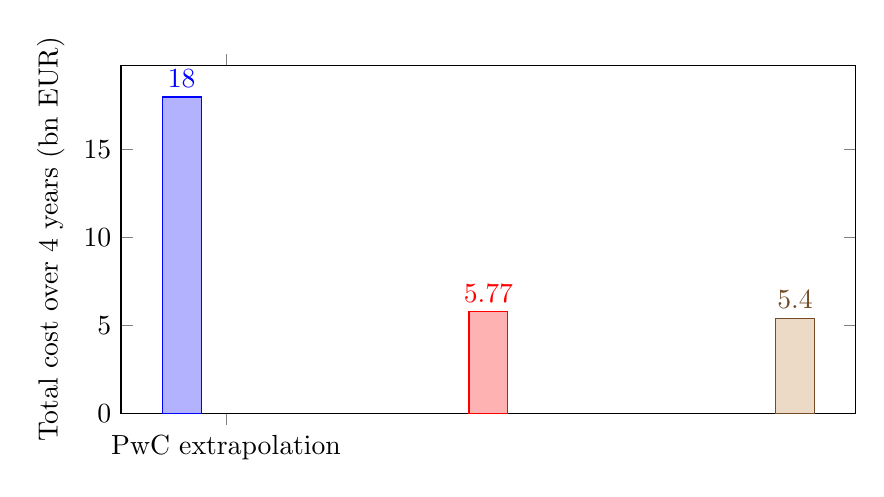
\begin{tikzpicture}
\begin{axis}[
  ybar,
  bar width=14pt,
  width=0.9\textwidth,
  height=6cm,
  ylabel={Total cost over 4 years (bn EUR)},
  symbolic x coords={PwC extrapolation,ECB synergy-adjusted range,EC impact assessment range},
  xtick=data,
  ymin=0,
  enlarge x limits=0.2,
  nodes near coords,
  nodes near coords align={vertical},
]
\addplot coordinates {(PwC extrapolation,18)};
\addplot coordinates {(ECB synergy-adjusted range,5.77)};
\addplot coordinates {(EC impact assessment range,5.4)};
\end{axis}
\end{tikzpicture}
\caption{Indicative total cost comparisons (upper bounds shown for ranges). Sources: \textcite{pwc_coststudy_2025} and \textcite{ecb_costs_2025}.}
\label{fig:cost-range}
\end{figure}

\section{IT spending context and capacity constraints}
Sector survey data for the Italian banking sector reports substantial aggregate ICT costs and a significant share of third-party spending, suggesting material reliance on external providers and supporting the plausibility of utility/shared-service models for new regulatory initiatives \parencite{cipa_rilevazione_it_2025}. The PwC study further highlights resource capacity constraints (skilled personnel share) as a key risk \parencite{pwc_coststudy_2025}.

% ============================================================
\chapter{Blueprints for bank-tier implementations}
This chapter provides concrete blueprints for the three implementation models and highlights module placement decisions.

\section{Blueprint A: Tier 1--2 hybrid platform}
\subsection{Key characteristics}
\begin{itemize}
\item Bank-operated DEIL on internal Kubernetes platform.
\item Shared gateway adapter and conformance harness procured from a vendor (or built once at group level).
\item Event-driven integration to AML/fraud and reporting; strict state machine service for payments.
\item Dedicated offline device management service shared across subsidiaries.
\end{itemize}

\subsection{Component placement}
\begin{table}[H]
\centering
\caption{Tier 1--2 hybrid blueprint: component ownership}
\begin{tabularx}{\textwidth}{@{}lXl@{}}
\toprule
Component & Description & Owner \\ \midrule
DEIL orchestration & Payment state machine, idempotency, retries, reconciliation & Bank \\
Gateway adapter & REST/gRPC client, signing, version mgmt, certification & Shared vendor/utility \\
AML/fraud connectors & Screening, monitoring, case management integration & Bank \\
Offline provisioning & SE lifecycle, key mgmt, counters, risk params & Shared (group/utility) \\
Channel UX & Wallet UI, merchant flows, notifications & Bank \\
\bottomrule
\end{tabularx}
\end{table}

\section{Blueprint B: Tier 3 hybrid-leaning-outsourced}
Mid-sized banks typically benefit from utility services for gateway adapter, offline and acceptance upgrades. Banks retain compliance/risk integration due to local policy requirements.

\section{Blueprint C: Tier 4 outsourced/utility model}
Tier 4 banks minimise fixed costs by:
\begin{itemize}
\item Consuming a hosted DEIL service (multi-tenant) plus shared gateway adapter.
\item Using centrally provided channel components where permitted (e.g., standard wallet UI) and integrating only customer servicing and compliance hooks.
\item Relying on merchant/acquirer utilities for acceptance upgrades and on ATM utilities for physical access paths.
\end{itemize}
This aligns with ECB emphasis that banks need not implement the digital euro on a stand-alone basis and can rely on shared solutions \parencite{ecb_costs_2025}.

% ============================================================
\chapter{Governance, risk, and compliance considerations}
\section{Regulatory alignment}
Legislative discussions emphasise that the digital euro would complement cash and provide payment functionality across the euro area \parencite{eu_council_2025_digital_euro_position}. Banks must implement in a way consistent with scheme rules and supervisory expectations around operational resilience.

\section{Operational resilience and DORA}
Digital euro integration extends the bank's critical payment perimeter. Key controls include:
\begin{itemize}
\item resilience-by-design (redundancy, failover, chaos testing),
\item third-party risk management (vendor due diligence, concentration risk),
\item incident response and reporting workflows,
\item secure SDLC and cryptographic key governance.
\end{itemize}

\section{Privacy and data protection}
While privacy design is partly scheme-defined, intermediaries control significant data surfaces: customer identity, transaction monitoring, and support logs. Architecture should implement data minimisation, strong access controls, and auditable processing consistent with GDPR principles.

% ============================================================
\chapter{Discussion}
\section{Answering the research questions}
\textbf{RQ1} is addressed via the DEIL-based reference architecture and integration patterns. \textbf{RQ2} is addressed via scheme vs intermediary responsibility mapping. \textbf{RQ3} is addressed through the component impact map and domain decomposition. \textbf{RQ4} is addressed through the mutualisation taxonomy, emphasising shared gateway/offline/acceptance utilities. \textbf{RQ5} is addressed through tiering, MCDA and blueprint recommendations.

\section{Limitations}
Rulebook details and technical specifications may evolve; therefore the architecture is designed to isolate scheme evolution behind adapters and versioning boundaries \parencite{ecb_rdg_progress_2025}. Cost estimates remain sensitive to design choices (offline scope, multiple accounts, acquiring).

\section{Future research}
Future work could: (i) validate the blueprint using empirical case studies with banks/PSPs, (ii) extend cost modelling with institution-specific parameters, (iii) evaluate interoperability reuse for private payment schemes.

% ============================================================
\chapter{Conclusion}
This thesis provides a rulebook-aligned reference architecture and a pragmatic operating-model framework for banks integrating the digital euro. Evidence suggests that while stand-alone implementations could be costly, significant cost mutualisation is feasible through shared services and utilities \parencite{ecb_costs_2025}. The recommended approach is tiered: large banks adopt hybrid/in-house architectures for strategic control and reuse, while smaller institutions leverage outsourced/utility models to reduce fixed costs and operational burden. Across all tiers, careful modularisation of gateway adapters, offline services, and acceptance infrastructure enables interoperability, resilience, and the potential to reuse digital euro standards for broader European payment innovation.

\cleardoublepage
\printbibliography

\appendix
\chapter{Appendix: PwC layer distribution chart}
Figure~\ref{fig:pwc-layer} shows an illustrative representation of the PwC reported cost-layer distribution (commercial/technical/operational).

\begin{figure}[H]
\centering
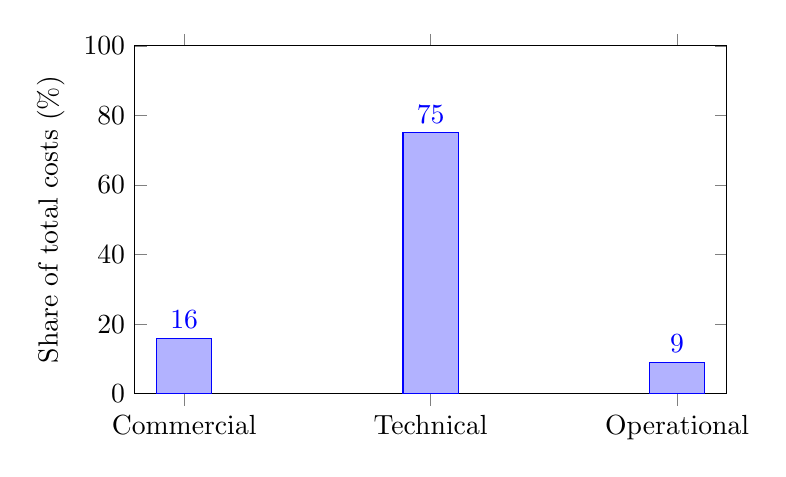
\begin{tikzpicture}
\begin{axis}[
  ybar,
  bar width=20pt,
  width=0.75\textwidth,
  height=6cm,
  ymin=0, ymax=100,
  ylabel={Share of total costs (\%)},
  symbolic x coords={Commercial,Technical,Operational},
  xtick=data,
  nodes near coords,
]
\addplot coordinates {(Commercial,16) (Technical,75) (Operational,9)};
\end{axis}
\end{tikzpicture}
\caption{Cost distribution across PwC payment layer model (reported shares). Source: \textcite{pwc_coststudy_2025}.}
\label{fig:pwc-layer}
\end{figure}

\chapter{Appendix: Practical checklist for banks}
\begin{enumerate}
\item Establish target operating model (in-house/hybrid/outsourced) and vendor strategy.
\item Build domain-aligned backlog: access, transaction, liquidity, offline, reporting.
\item Stand up DEIL boundary: API gateways, signing, versioning, test harness.
\item Integrate treasury/DCA processes and limit controls.
\item Integrate AML/fraud monitoring and customer support workflows.
\item Plan acceptance upgrades (POS/ATM) with utilities; align with replacement cycles.
\item Execute conformance testing and operational readiness (BCP, incident response).
\end{enumerate}

\end{document}
